\documentclass[12pt,letterpaper,twoside]{hmcpset}
\usepackage[margin=1in]{geometry}
\usepackage{graphicx}
\usepackage{commons}
\usepackage{algpseudocode}
\usepackage{tikz}
\usetikzlibrary{arrows}

% info for header block in upper right hand corner
\name{Zachary Seymour}
\class{CS 575}
\assignment{Theory Assignment 6}
\duedate{December 5, 2013}

\begin{document}
\begin{problem}[1]
 Find the longest subsequence for the strings $X = $C G C T A C C G and $Y =$A T C T G T A A C T G.  Show the table with the lengths and arrows.
\end{problem}

\begin{solution}
 \begin{center}
\begin{tabular}[c]{|l|l|l|l|l|l|l|l|l|l|l|l|l|}\hline
× & y & A & T & C & T & G & T & A & A & C & T & G\\\hline
x & 0 & 0 & 0 & 0 & 0 & 0 & 0 & 0 & 0 & 0 & 0 & 0\\\hline
C & 0 & $\leftarrow$ 0 & $\leftarrow$ 0 & $\nwarrow$ 1 & $\leftarrow$ 1 & $\leftarrow$ 1 & $\leftarrow$ 0 & $\leftarrow$ 1 & $\leftarrow$ 1 & $\nwarrow$ 1 & $\leftarrow$ 1  & $\leftarrow$ 1 \\\hline
G & 0 & $\uparrow$ 0 & $\uparrow$ 0 & $\uparrow$ 1 & $\uparrow$ 1 & $\nwarrow$ 2 & $\leftarrow$ 2 & $\leftarrow$ 2 & $\leftarrow$ 2 & $\leftarrow$ 2 & $\leftarrow$ 2 & $\nwarrow$ 2\\\hline
C & 0 & $\uparrow$ 0 & $\uparrow$ 0 & $\nwarrow$ 1 & $\leftarrow$ 1 & $\uparrow$ 2  & $\leftarrow$ 2 & $\leftarrow$ 2 & $\leftarrow$ 2 & $\nwarrow$ 3 & $\leftarrow$ 3 & $\leftarrow$ 3\\\hline
T & 0 & $\uparrow$ 0 & $\nwarrow$ 1 & $\leftarrow$ 1 & $\nwarrow$ 2 & $\leftarrow$ 2 & $\nwarrow$ 3 & $\leftarrow$ 3 & $\leftarrow$ 3  & $\leftarrow$ 3  & $\nwarrow$ 4 & $\leftarrow$ 4\\\hline
A & 0 & $\nwarrow$ 1 & $\leftarrow$ 1 & $\leftarrow$ 1 & $\uparrow$ 2 & $\leftarrow$ 2 & $\uparrow$ 3 & $\nwarrow$ 4 & $\nwarrow$ 4 & $\leftarrow$ 4 & $\leftarrow$ 4 & $\leftarrow$ 4\\\hline
C & 0 & $\uparrow$ 1 & $\leftarrow$ 1 & $\nwarrow$ 2 & $\leftarrow$ 2 & $\leftarrow$ 2 & $\uparrow$ 3 & $\uparrow$ 4 & $\uparrow$ 4 & $\nwarrow$ 5 & $\leftarrow$ 5 & $\leftarrow$ 5\\\hline
C & 0 & $\uparrow$ 1 & $\leftarrow$ 1 & $\nwarrow$ 2 & $\leftarrow$ 2 & $\leftarrow$ 2 & $\uparrow$ 3 & $\uparrow$ 4 & $\uparrow$ 4 & $\nwarrow$ 5 & $\leftarrow$ 5 & $\leftarrow$ 5\\\hline
G & 0 & $\uparrow$ 1 & $\leftarrow$ 1  & $\uparrow$ 2 & $\leftarrow$ 2 & $\nwarrow$ 3 & $\leftarrow$ 3 & $\uparrow$ 4 & $\leftarrow$ 4 & $\uparrow$ 5 & $\leftarrow$ 5 & $\nwarrow$ 6\\\hline
 \end{tabular}
 \end{center}


The longest subsequence is, then, C G T A C G.
\end{solution}


\begin{problem}[2]
 Given the following 5 matrices A1 with 30 rows and 35 columns, A2 with 35 rows and 15 columns, A3 with 15 rows and 5 columns, A4 with 5 rows and 10 columns, A5 with 10 rows and 20 columns.  Compute the diagonal matrix with the minimum number of multiplications, and the factor matrix used to determine the multiplication order. 
\end{problem}

\begin{solution}
The matrix of diagonals:
\[
\begin{bmatrix}
0 & 36750 & 34125 & 40875 & 15125 & 15500 & 16875 & 17375 & 19875\\
0 & 0 & 18375 & 26250 & 9875 & 10250 & 11875 & 12375 & 151125\\
0 & 0 & 0 & 7875 & 3750 & 4125 & 5750 & 6250 & 9000\\
0 & 0 & 0 & 0 & 1125 & 1500 & 2125 & 2625 & 4375\\
0 & 0 & 0 & 0 & 0 & 375 & 1000 & 1500 & 3250\\
0 & 0 & 0 & 0 & 0 & 0 & 250 & 750 & 1750\\
0 & 0 & 0 & 0 & 0 & 0 & 0 & 500 & 1500\\
0 & 0 & 0 & 0 & 0 & 0 & 0 & 0 & 2000\\
0 & 0 & 0 & 0 & 0 & 0 & 0 & 0 & 0
\end{bmatrix}
\]

The factor matrix:
\[
\begin{bmatrix}
0 & 0 & 0 & 2 & 0 & 0 & 4 & 4 & 4\\
0 & 0 & 1 & 1 & 1 & 1 & 4 & 4 & 4\\
0 & 0 & 0 & 2 & 2 & 2 & 4 & 4 & 4\\
0 & 0 & 0 & 0 & 3 & 3 & 4 & 4 & 4\\
0 & 0 & 0 & 0 & 0 & 4 & 4 & 4 & 4\\
0 & 0 & 0 & 0 & 0 & 0 & 5 & 5 & 7\\
0 & 0 & 0 & 0 & 0 & 0 & 0 & 6 & 7\\
0 & 0 & 0 & 0 & 0 & 0 & 0 & 0 & 7\\
0 & 0 & 0 & 0 & 0 & 0 & 0 & 0 & 0
\end{bmatrix}
\]

\end{solution}


\begin{problem}[3]
 Find the shortest distance between all pairs of nodes in the following graph.  Show the matrices $D^0, D^1,\dotsc,D^4$.
 
 \centering
 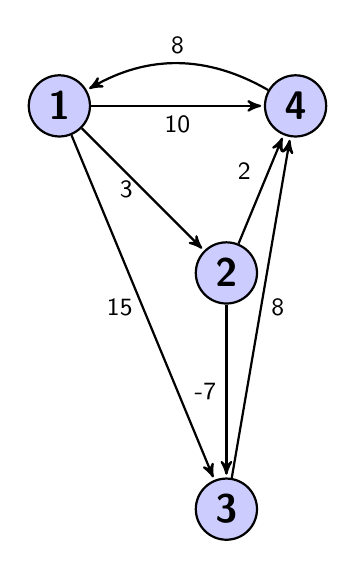
\begin{tikzpicture}[->,>=stealth',shorten >=1pt,auto,node distance=3cm,
  thick,main node/.style={circle,fill=blue!20,draw,font=\sffamily\Large\bfseries}]

  \node[main node] (1) {1};
  \node[main node] (2) [below right of=1] {2};
  \node[main node] (3) [below of=2] {3};
  \node[main node] (4) [right of=1] {4};

  \path[every node/.style={font=\sffamily\small}]
    (1) edge node [below] {10} (4)
        edge node[left] {3} (2)
        edge node[left] {15} (3)
    (2) edge node {2} (4)
        edge node[left] {-7} (3)
    (3) edge node[right] {8} (4)
    (4) edge [bend right] node[above] {8} (1);
\end{tikzpicture}
\end{problem}

\begin{solution}
\[
 \begin{aligned}
    D^0 = W &=\begin{bmatrix}0 & 3 & 15 & 10\\\infty & 0 & -7 & 2\\\infty & \infty & 0 & 8\\8 & \infty & \infty & 0\end{bmatrix} \\
    D^1 &= \begin{bmatrix}0 & 3 & 15 & 10\\\infty & 0 & -7 & 2\\\infty & \infty & 0 & 8\\8 & 11 & 23 & 0          \end{bmatrix}\\
    D^2 &= \begin{bmatrix}0 & 3 & -4 & 5\\\infty & 0 & -7 & 2\\\infty & \infty & 0 & 8\\8 & 11 & 4 & 0           \end{bmatrix}\\
    D^3 &= \begin{bmatrix}0 & 3 & -4 & 4\\\infty & 0 & -7 & 1\\\infty & \infty & 0 & 8\\8 & 11 & 4 & 0           \end{bmatrix}\\
    D^4 = D &=\begin{bmatrix}0 & 3 & -4 & 4\\9 & 0 & -7 & 1\\16 & 19 & 0 & 8\\8 & 11 & 4 & 0              \end{bmatrix}
 \end{aligned}
\]
\end{solution}

\begin{problem}[4]
 How can the output of the Floyd-Warshall algorithm be used to detect the presence of a negative weight cycle?
\end{problem}

\begin{solution}
A negative cycle in the graph would indicate a path from a node $i$ to itself with negative length.  Thus, when inspecting the diagonal entries of the matrix produced from the algorithm, any negative entries will indicate the existence of a negative cycle.
\end{solution}

\begin{problem}[5]
 Give a memoized version of the longest common subsequence that runs in $\BigO{mn}$ time.
\end{problem}

\begin{solution}
 \begin{algorithmic}
  \Function{Initialize}{x,y}
  \State m $\leftarrow$ length(x)
  \State n $\leftarrow$ length(y)
  \For{i = 0 to m}
    \State c[i,0] $\leftarrow$ 0
  \EndFor
  \For{j = 0 to n}
    \State c[0,j] $\leftarrow$ 0
  \EndFor
  \Comment initialize memoization matrix
  \For{i = 0 to m}
    \For{j = 0 to n}
      \State l[i,j] = -1
    \EndFor
  \EndFor
  \State\Return LCS-LENGTH(m,n)
  \EndFunction
  \Function{LCS-Length}{i,j}
  
  \If{i$=0$ or j$=0$}
    \State\Return 0
  \EndIf
  
  \If{l[i,j]$\geq$0}
    \State\Return l[i,j]
  \EndIf
  
  \If{x$_{i-1}$ = y$_{i-1}$}
    \State len = LCS-LENGTH{i-1, j-1}
    \State l[i,j] = len + 1
    \State b[i,j] = ``D''
    \State\Return len + 1
  \Else
    \State len1 = LCS-LENGTH(i-1,j) 
    \State len2 = LCS-LENGTH(i,j-1)
    \If{len1 $\geq$ len2}
      \State l[i,j] = len1
      \State b[i,j] = ``U''
      \State\Return len1
    \Else
      \State l[i,j] = len2
      \State b[i,j] = ``L''
      \State\Return len2
    \EndIf
  \EndIf
  
  \EndFunction
 \end{algorithmic}

\end{solution}

\begin{problem}[6a]
 Apply the greedy algorithm for 0/1 integer knapsack that chooses the next items with the highest b/w, to the following problem.  $W=11$ and there are 4 items.  The weights and benefits are shown in the table below.
\begin{center}
 \begin{tabular}{|l|l|l|l|l|}\hline
Item & 1 & 2 & 3 & 4\\\hline
w & 1 & 2 & 10 & 6\\\hline
b & 1 & 4 & 36 & 24\\\hline
 \end{tabular}
\end{center}


\end{problem}

\begin{solution}
 We choose Item 4, Item 2, and Item 1, in that order, for a weight of 9 and a benefit of 29.
\end{solution}

\begin{problem}[6b]
 Apply KWF to this problem
\end{problem}

\begin{solution}
 We add Item 4 and half of Item 3, for a weight of 11 and a benefit of 42.
\end{solution}

\begin{problem}[6c]
 Apply the dynamic programming algorithm to the problem.
\end{problem}

\begin{solution}
\setcounter{MaxMatrixCols}{20}
 \[
\begin{bmatrix}
0 & 0 & 0 & 0 & 0 & 0 & 0 & 0 & 0 & 0 & 0 & 0\\
0 & 1 & 1 & 1 & 1 & 1 & 1 & 1 & 1 & 1 & 1 & 1\\
0 & 1 & 5 & 6 & 6 & 6 & 6 & 6 & 6 & 6 & 6 & 6\\
0 & 1 & 5 & 6 & 6 & 6 & 6 & 6 & 6 & 36 & 37 & 42\\
0 & 1 & 5 & 6 & 6 & 6 & 24 & 25 & 29 & 30 & 30 & 30
\end{bmatrix}
 \]

\end{solution}


\end{document}
